\documentclass[11pt]{article}

\usepackage[margin=1in]{geometry}
\usepackage{amsmath,amssymb,amsthm,mathtools}
\usepackage{bm}
\usepackage{hyperref}
\usepackage{enumitem}
\usepackage{booktabs}
\usepackage{tikz}
\usepackage{xcolor}
\usepackage{mdframed}
\usepackage{tcolorbox}

\hypersetup{colorlinks=true,linkcolor=blue,citecolor=blue,urlcolor=blue}
\setlist[itemize]{leftmargin=2em}
\setlist[enumerate]{leftmargin=2.2em}

% -------- notation shortcuts --------
\newcommand{\PP}{\mathbb{P}}
\newcommand{\QQ}{\mathbb{Q}}
\newcommand{\EE}{\mathbb{E}}
\newcommand{\FF}{\mathcal{F}}
\newcommand{\NN}{\mathcal{N}}
\newcommand{\R}{\mathbb{R}}
\newcommand{\dd}{\,\mathrm{d}}

% coloured insight boxes
\tcbuselibrary{skins,breakable}
\newtcolorbox{intuition}[1][]{
  colback=blue!5!white, colframe=blue!50!black,
  title=\textbf{Intuition}, fonttitle=\bfseries, #1, breakable}
\newtcolorbox{example_box}[1][]{
  colback=green!5!white, colframe=green!50!black,
  title=\textbf{Worked Example}, fonttitle=\bfseries, #1, breakable}
\newtcolorbox{recall_box}[1][]{
  colback=orange!5!white, colframe=orange!60!black,
  title=\textbf{Recall from Class}, fonttitle=\bfseries, #1, breakable}

\title{\textbf{Term Project: First Draft}\\
\large Short-Rate Modeling, Term Structure, and Interest Rate Derivatives\\
\normalsize MATH 60646A -- Stochastic Calculus, HEC Montr\'eal, Winter 2026}
\author{}
\date{\today}

\begin{document}
\maketitle
\tableofcontents
\newpage

%------------------------------------------------------------
\section*{A Note on How to Read This Document}
%------------------------------------------------------------

This document is written the way an instructor would write notes: every
mathematical object is introduced in plain language before any formula
appears, every formula is translated back into plain language after it is
written, and every key idea is illustrated with at least one concrete
example.  We work throughout on a filtered probability space
$(\Omega,\FF,(\FF_t)_{t\ge 0},\PP)$, where $\PP$ is the physical
(real-world) probability measure.  The risk-neutral measure will be
denoted $\QQ$.  We recall key definitions from the course as we need them
so that this document is self-contained.

\textbf{Assumption convention.}  At the start of each section we state
explicitly which measure we are working under, which filtration we are
conditioning on, and what technical assumptions are in force.  This is
crucial: the same equation can mean different things under $\PP$ and $\QQ$.

\newpage
%============================================================
\section{Question 2: Spot rate, forward rate, and the zero-coupon yield curve}
%============================================================

\subsection{Starting from scratch: why do we need a yield curve at all?}

Imagine you are a pension fund manager in January 2026 and you need to
invest cash for 10 years.  A bank offers you $3\%$ per year.  Is that a
good deal?  You cannot answer that question without knowing what
\emph{other} rates are available for different maturities right now.  The
collection of all such rates -- one rate for every maturity $T$ -- is what
we call the \textbf{yield curve} (or the term structure of interest rates).
It is, literally, the price of time.

Fixed-income mathematics is built on one primitive object: the
\textbf{zero-coupon bond}.  Everything else -- yield curves, forward rates,
swaps, swaptions -- is ultimately expressed in terms of zero-coupon bond
prices.  So we start there.

\subsection{The zero-coupon bond}

A \textbf{zero-coupon bond with maturity $T$} is a contract that pays
exactly \$1 at time $T$ and nothing before.  There are no coupon payments,
no dividends, no intermediate cash flows -- just one dollar at one future
date.  We denote its price at time $t \le T$ by $P(t,T)$.

\begin{example_box}
\textbf{Concrete example.}  Suppose it is time $t = 0$ (today) and a
one-year zero-coupon bond trades at $P(0,1) = 0.95$.  This means: to
receive \$1.00 in exactly one year, you must pay \$0.95 today.  The
\emph{cost of waiting} one year is $1/0.95 - 1 \approx 5.26\%$ in simple
terms.  This is the market's current price for time value over one year.

Now suppose a two-year bond trades at $P(0,2) = 0.88$.  You pay \$0.88
today to receive \$1.00 in two years.  The annualised cost of waiting is
$(1/0.88)^{1/2} - 1 \approx 6.6\%$.

Notice two things:
\begin{enumerate}
  \item $P(0,T)$ is \emph{decreasing} in $T$: the longer you wait, the
  less you pay today, because your money is locked up longer.
  \item $P(t,T) \in (0,1]$ for $T \ge t$ under positive interest rates:
  the present value of \$1 in the future is always less than \$1 today.
  \item $P(t,t) = 1$ always: a bond that matures right now is worth
  exactly what it pays, which is \$1.
\end{enumerate}
\end{example_box}

\subsection{The zero-coupon yield $y(t,T)$}

Given the bond price $P(t,T)$, we define the \textbf{continuously
compounded zero-coupon yield} $y(t,T)$ as the constant rate that makes the
discounting identity exact:
\[
P(t,T) = e^{-y(t,T)(T-t)}.
\]
Solving for $y$:
\[
y(t,T) = -\frac{1}{T-t}\log P(t,T).
\]

\begin{intuition}
Think of $y(t,T)$ as the answer to the question: ``\emph{If I could earn a
single constant interest rate from $t$ to $T$, what rate would give me the
same bond price?}''  It is a \emph{summary statistic} of the entire bond
price in one number.  When people say ``the 10-year yield is 4\%'', they
are referring to this: $y(\text{today}, \text{today}+10) = 4\%$.
\end{intuition}

\begin{example_box}
Using our numbers above:
\[
y(0,1) = -\log(0.95) \approx 0.0513 = 5.13\%.
\]
\[
y(0,2) = -\frac{1}{2}\log(0.88) \approx 0.0645 = 6.45\%.
\]
Because $y(0,2) > y(0,1)$, the yield curve is \emph{upward sloping}: you
demand a higher annualised return for tying your money up for two years
instead of one.  This is the most common shape in normal economic times,
reflecting both expected future rate increases and a term premium for
bearing duration risk.
\end{example_box}

The function $T \mapsto y(t,T)$, plotted for all maturities $T > t$, is the
\textbf{zero-coupon yield curve at time $t$}.  It encodes everything the
market ``believes'' (under the risk-neutral measure) about future interest
rates.

\subsection{The instantaneous forward rate $f(t,T)$}

The yield $y(t,T)$ is an \emph{average} rate over the whole period
$[t,T]$.  But sometimes we want to know the \emph{marginal} rate: ``what
is the market implying for the cost of borrowing for an infinitesimally
short interval around a specific future date $T$?''  This is the
\textbf{instantaneous forward rate} $f(t,T)$.

Formally, it is the negative of the maturity-derivative of the log bond
price:
\[
f(t,T) := -\frac{\partial}{\partial T} \log P(t,T).
\]

\begin{intuition}
Here is the best way to think about this.  Imagine you are standing at
time $t$ and you hold a curve of bond prices $P(t,T)$ for all maturities.
The forward curve $T \mapsto f(t,T)$ is like the \emph{slope} of that
log-price curve, negated.  A steeply declining log-price curve means
high forward rates; a flatter curve means low forward rates.

More concretely: $f(t,T)\,\Delta T$ is approximately the rate you would
pay, locked in today, for borrowing from time $T$ to time $T+\Delta T$.
It is a ``futures rate'' in continuous time.
\end{intuition}

\begin{example_box}
Continuing our example, suppose the yield curve is smooth and given by
$y(0,T) = 0.04 + 0.01\sqrt{T}$ (just a made-up shape to get numbers).
Then
\[
\log P(0,T) = -y(0,T)\cdot T = -(0.04T + 0.01T^{3/2}),
\]
\[
f(0,T) = -\frac{\partial}{\partial T}\log P(0,T) = 0.04 + 0.015\sqrt{T}.
\]
At $T=1$: $f(0,1)=0.055$.  At $T=4$: $f(0,4)=0.07$.  So the forward
curve says: the cost of borrowing for one instant at year 4 is $7\%$.
Compare $y(0,4) = 0.04+0.01\times 2 = 0.06 = 6\%$.  The forward rate is
\emph{above} the yield at every maturity when the yield curve is
upward-sloping.  We will see why momentarily.
\end{example_box}

\subsection{Recovering the bond price from the forward curve}

Integrating $f(t,T) = -\partial_T \log P(t,T)$ over $[t,T]$ and using
$P(t,t) = 1$:
\[
\int_t^T f(t,u)\,\dd u
= -\log P(t,T) + \log P(t,t) = -\log P(t,T).
\]
Rearranging:
\[
\boxed{P(t,T) = \exp\!\left(-\int_t^T f(t,u)\,\dd u\right).}
\]
\textbf{In plain English:} the zero-coupon bond price at time $t$ for
maturity $T$ is the exponential of minus the area under the forward curve
from $t$ to $T$.  If you integrate all the future instantaneous rates
(forward rates) that the market prices today, you get the discount factor.
This is exactly analogous to how, in the deterministic case, the discount
factor is $e^{-rT}$ for a flat rate $r$ -- here the ``rate'' is not flat
but depends on maturity.

\subsection{Yield as the average of the forward curve}

Substituting the integral representation into the definition of $y(t,T)$:
\[
y(t,T)
= -\frac{\log P(t,T)}{T-t}
= \frac{1}{T-t}\int_t^T f(t,u)\,\dd u.
\]
\textbf{In plain English:} the zero-coupon yield for maturity $T$ is the
simple (maturity-weighted) average of the instantaneous forward rates
between $t$ and $T$.  This is why the yield curve is ``smoother'' than the
forward curve: it averages out the peaks and troughs.

\begin{intuition}
This averaging relationship is the key to understanding yield curve
shapes.  When the forward curve is above the yield curve (as in our
example), the yield curve is rising.  When the forward curve is below the
yield curve, the yield curve is falling.  When the forward curve crosses
the yield curve from above, the yield curve has a local maximum.  You can
always read the forward curve as ``the marginal slope information'' hidden
inside the yield curve.
\end{intuition}

\subsection{The instantaneous short rate $r_t$}

The \textbf{instantaneous short rate} $r_t$ is the limit of the forward
rate as the horizon collapses to zero:
\[
r_t = \lim_{T \downarrow t} y(t,T) = \lim_{T \downarrow t} f(t,T) = f(t,t).
\]
In other words, $r_t$ is the ``overnight'' (or more precisely,
infinitesimally short) rate of return on riskless lending at time $t$.  It
is the rate at which the \textbf{money-market account} $B_t$ accumulates:
\[
B_t = \exp\!\left(\int_0^t r_s\,\dd s\right), \qquad
\frac{\dd B_t}{B_t} = r_t\,\dd t.
\]
Unlike $y(t,T)$ and $f(t,T)$, which are observable from market prices, $r_t$
is typically \emph{not} directly observable -- it must be modelled or
inferred.  This is precisely why we need a \emph{short-rate model} (such as
CIR, which we study next).

\begin{example_box}
\textbf{Summary of relationships.}  Suppose at $t=0$ the following is
observed: $P(0,1)=0.95$, $P(0,2)=0.88$, $P(0,3)=0.80$.  Then:
\begin{align*}
y(0,1) &= -\log(0.95) \approx 5.13\% \\
y(0,2) &= -\tfrac{1}{2}\log(0.88) \approx 6.45\% \\
y(0,3) &= -\tfrac{1}{3}\log(0.80) \approx 7.44\%
\end{align*}
The average forward rate from 0 to 2 equals $y(0,2)=6.45\%$.  The forward
rate for the second year alone is obtained by ``stripping'':
\[
P(0,2) = P(0,1)\cdot e^{-f(0;1,2)\cdot 1}
\implies f(0;1,2) = \log P(0,1) - \log P(0,2) = \log\frac{0.95}{0.88} \approx 7.7\%.
\]
So the market is implying a $7.7\%$ rate for year two.  Notice this is
higher than both $y(0,1)$ and $y(0,2)$ precisely because the yield curve
is upward sloping.
\end{example_box}

\subsection{Static conceptual graph}

\begin{figure}[ht]
\centering
\begin{tikzpicture}[scale=1.1]
  \draw[->] (0,0) -- (8.5,0) node[right] {Maturity $T$};
  \draw[->] (0,0) -- (0,4.5) node[above] {Rate (\%)};
  % yield curve
  \draw[thick,blue] plot[smooth] coordinates
    {(0.2,1.5)(1.0,1.8)(2.0,2.3)(3.2,2.7)(4.5,3.0)(6.0,3.2)(7.8,3.35)};
  % forward curve
  \draw[thick,red,dashed] plot[smooth] coordinates
    {(0.2,1.5)(1.0,2.1)(2.0,3.0)(3.2,3.4)(4.5,3.65)(6.0,3.75)(7.8,3.8)};
  % r_0 dot
  \fill[black] (0.2,1.5) circle (2pt) node[left] {$r_0$};
  % labels
  \node[blue] at (7.2,2.8) {$y(0,T)$};
  \node[red] at (7.2,4.1) {$f(0,T)$};
  % arrows and annotations
  \draw[<->] (3.2,2.7) -- (3.2,3.4) node[midway,right,font=\footnotesize]
    {forward $>$ yield};
\end{tikzpicture}
\caption{An upward-sloping yield curve and its associated forward curve at $t=0$.
The forward curve lies above the yield curve wherever the yield curve is
increasing (because you are pulling the average up from the right).  Both
curves pass through $r_0$ at the short end, since for vanishing maturities
$y(0,T)\to r_0$ and $f(0,T)\to r_0$.  When the yield curve is downward
sloping the positions reverse: the forward curve dips below the yield
curve.}
\end{figure}

\subsection{Why does the yield curve have a ``shape'' at all?}

A natural question: if we observe yield curves every day, why do they
slope up on some days and down on others?  There are two forces at work:

\begin{enumerate}
  \item \textbf{Expectations:} If the market believes short rates will rise,
  long yields must be higher today to compensate (otherwise everyone
  would park money short-term and roll it over at higher rates).
  \item \textbf{Risk premium:} Longer bonds are riskier (more sensitive to
  rate changes), so investors demand a premium -- a term premium -- for
  holding them.
\end{enumerate}

Under the physical measure $\PP$, both effects contribute.  Under the risk-neutral
measure $\QQ$, the risk premium is absorbed into the drift of $r_t$, and the
yield curve reflects only the $\QQ$-expected path of future short rates.
We will make this precise in Questions 3 and 4.

\subsection{Simulation ideas for iteration 2}
\begin{itemize}
  \item Interactive dashboard: given parameters of a CIR model, plot $y(0,T)$,
  $f(0,T)$, and $P(0,T)$ as maturity $T$ varies.
  \item Slider for $r_0$, $\kappa_{\QQ}$, $\theta_{\QQ}$, $\sigma$ showing
  how the term structure responds.
  \item Historical: load FRED data for two dates (one normal, one inverted
  curve) and plot both yield and forward curves side by side.
\end{itemize}

\subsection*{Open-ended questions}
\begin{itemize}
  \item An \emph{inverted} yield curve (short rates above long rates) has
  historically preceded recessions.  Can you explain why, using the
  expectations component above?
  \item What happens to the forward rate $f(t,T)$ as $T \to \infty$?
  Does it always converge?  What does convergence (or divergence) imply
  about the model?
\end{itemize}

\newpage
%============================================================
\section{Question 3: Short-rate dynamics under $\PP$ (CIR model)}
%============================================================

\subsection{Recall: the probability space and measure $\PP$}

\begin{recall_box}
From our course (Definition 5, Reminder sheet), a \textbf{probability
measure} $\PP$ on a measurable space $(\Omega,\FF)$ is a function
$\PP:\FF\to[0,1]$ satisfying $\PP(\Omega)=1$, nonnegativity, and
countable additivity.  The triple $(\Omega,\FF,\PP)$ is a
\textbf{probability space}.

In financial modelling, $\PP$ is the \textbf{physical} (or
\textbf{real-world}) measure: it is the probability measure that governs
what actually happens in the economy.  If you estimated interest rate
dynamics from 20 years of daily Fed Funds data and fitted a model, you
would be working under $\PP$.

From Definition 6, a \textbf{filtration} $(\FF_t)_{t\ge 0}$ is an
increasing family of $\sigma$-algebras, with $\FF_s \subseteq \FF_t$ for
$s \le t$.  We interpret $\FF_t$ as ``all information available up to and
including time $t$''.
\end{recall_box}

\subsection{What is a standard Brownian motion under $\PP$?}

A \textbf{standard Brownian motion under $\PP$}, written $W_t^\PP$, is a
continuous-time stochastic process (a family of random variables indexed
by time) satisfying:
\begin{enumerate}
  \item $W_0^\PP = 0$ (starts at zero),
  \item \textbf{Independent increments:} for $0\le s< t$, $W_t^\PP - W_s^\PP$ is
  independent of $\FF_s$ (the future is unpredictable given today),
  \item \textbf{Gaussian increments:} $W_t^\PP - W_s^\PP \sim \NN(0, t-s)$
  (the increment is normally distributed with variance equal to the
  elapsed time),
  \item \textbf{Continuous paths:} the sample paths $t\mapsto W_t^\PP(\omega)$
  are continuous with probability one.
\end{enumerate}

\begin{intuition}
Think of $W_t^\PP$ as the ``cumulative surprise'' accumulated by time $t$.
At each instant, a tiny shock $\dd W_t^\PP \sim \NN(0,\dd t)$ arrives.
These shocks are independent and have no memory.  The variance of the total
accumulated shock grows linearly with time: $\mathrm{Var}^\PP[W_t^\PP]=t$.

The phrase ``under $\PP$'' tells you which probability measure is
generating the distribution.  This will matter enormously when we switch
to $\QQ$: the same process $W_t^\PP$ will \emph{not} be a Brownian motion
under $\QQ$ (it will have a drift).  This is the content of Girsanov's
theorem, which we revisit in Question 4.
\end{intuition}

\subsection{Why do we need a stochastic model for the short rate?}

Before we write down the CIR model, let us ask: \emph{why not just use a
deterministic interest rate?}  After all, central banks announce rates in
advance.

The answer is that interest rates are genuinely random over horizons longer
than a few weeks.  No one in January 2021 predicted that the US Federal
Funds rate would go from $0.25\%$ to $5.33\%$ in eighteen months.  A
deterministic model would price a 10-year bond incorrectly, and it would
assign zero value to interest rate derivatives (options on rates), which is
clearly wrong.  We need a model that:
\begin{itemize}
  \item Generates a distribution of possible future rates (not just one path),
  \item Keeps rates non-negative (nominal rates have historically been
  non-negative in most markets),
  \item Captures \emph{mean reversion} -- rates tend to drift back toward a
  long-run level rather than wandering off to infinity or zero,
  \item Is tractable enough to price bonds and derivatives in closed or
  semi-closed form.
\end{itemize}

\subsection{The CIR square-root diffusion}

The \textbf{Cox--Ingersoll--Ross (CIR) model} (1985) specifies that the
short rate $r_t$ under $\PP$ satisfies the stochastic differential equation:
\[
\dd r_t = \kappa_\PP\!\left(\theta_\PP - r_t\right)\dd t
+ \sigma\sqrt{r_t}\,\dd W_t^\PP, \qquad r_0 > 0.
\]

Let us immediately unpack every piece of this equation, term by term.

\paragraph{The drift term: $\kappa_\PP(\theta_\PP - r_t)\,\dd t$.}
This is a \textbf{mean-reverting} (Ornstein-Uhlenbeck-type) drift.  Let us
see why.
\begin{itemize}
  \item If $r_t < \theta_\PP$, then $\theta_\PP - r_t > 0$, so the drift is
  \emph{positive}: the rate is pulled \emph{upward} toward $\theta_\PP$.
  \item If $r_t > \theta_\PP$, then $\theta_\PP - r_t < 0$, so the drift is
  \emph{negative}: the rate is pushed \emph{downward} toward $\theta_\PP$.
  \item If $r_t = \theta_\PP$, the drift is exactly zero: no systematic pull.
\end{itemize}
The parameter $\kappa_\PP > 0$ controls \emph{how fast} this pull happens.
A large $\kappa_\PP$ means quick reversion (the rate snaps back rapidly); a
small $\kappa_\PP$ means slow reversion (the rate wanders widely before
returning).

\paragraph{The long-run level: $\theta_\PP$.}
This is the value toward which $r_t$ is pulled.  Economically, it
represents the steady-state level of the short rate in the physical world --
think of it as the ``normal'' interest rate environment.

\paragraph{The diffusion term: $\sigma\sqrt{r_t}\,\dd W_t^\PP$.}
This injects randomness.  The key feature is that the volatility is
\textbf{state-dependent}: it is proportional to $\sqrt{r_t}$.

Why $\sqrt{r_t}$ and not just a constant $\sigma$?  Two reasons:
\begin{enumerate}
  \item When $r_t$ is close to zero, $\sqrt{r_t} \approx 0$, so the
  stochastic part is very small.  Combined with the positive drift
  $\kappa_\PP\theta_\PP$ at the boundary, this keeps $r_t \ge 0$.
  \item Empirically, interest rate volatility \emph{does} tend to be higher
  when rates are higher (e.g., the volatile high-rate environments of the
  1980s).  The $\sqrt{r_t}$ specification captures this heteroscedasticity.
\end{enumerate}

\begin{example_box}
\textbf{Intuitive parameter choices.}  Suppose we calibrate to US data and
find $\kappa_\PP = 0.3$, $\theta_\PP = 0.04$ (4\%), $\sigma = 0.05$,
$r_0 = 0.02$ (2\%).

\begin{itemize}
  \item \textbf{Half-life of reversion:} The mean reversion half-life is
  $\log(2)/\kappa_\PP = \log(2)/0.3 \approx 2.3$ years.  So if rates start
  at 2\%, they will be approximately halfway back to 4\% after 2.3 years on
  average.
  \item \textbf{Instantaneous volatility at $r_0=0.02$:}
  $\sigma\sqrt{r_0} = 0.05\sqrt{0.02} \approx 0.007$ per year, i.e., 70
  basis points per year of standard deviation.
  \item \textbf{Volatility at $r=0.08$:}
  $0.05\sqrt{0.08} \approx 0.014$, double the volatility at 2\%.  Higher
  rates come with more noise, which is realistic.
\end{itemize}
\end{example_box}

\subsection{(i) Why does this model admit a strong solution?}

\paragraph{Weak vs.\ strong solutions.}  There are two notions of
``solution'' to an SDE $\dd X_t = b(X_t)\dd t + \sigma(X_t)\dd W_t$.
\begin{itemize}
  \item A \textbf{weak solution} is a triplet (probability space, Brownian
  motion, adapted process) satisfying the SDE.  You get to \emph{choose}
  the probability space and Brownian motion.
  \item A \textbf{strong solution} is an adapted process built on a
  \emph{given} probability space with a \emph{given} Brownian motion,
  satisfying the SDE pathwise (i.e., almost surely for every $\omega$).
  You must \emph{work with the Brownian motion you are handed}.
\end{itemize}
A strong solution is more demanding.  If a strong solution exists and is
unique (pathwise uniqueness), we say the SDE is \emph{well-posed}.

\paragraph{Standard sufficient conditions.} The classical result
(It\^{o}, 1951) is: if $b$ and $\sigma$ are globally \textbf{Lipschitz
continuous} and have \textbf{linear growth}, then there exists a unique
strong solution.  For CIR:
\begin{itemize}
  \item Drift: $b(r) = \kappa_\PP(\theta_\PP - r)$.  This is linear in $r$,
  hence globally Lipschitz.  Check: $|b(r_1)-b(r_2)| = \kappa_\PP|r_1-r_2|$.
  \item Diffusion: $a(r) = \sigma\sqrt{r}$.  This is \textbf{H\"older-}$\tfrac{1}{2}$
  but \emph{not} Lipschitz near $r=0$, because
  $|\sqrt{r_1}-\sqrt{r_2}| \le \sqrt{|r_1-r_2|}$, which is
  sublinear but not linear.
\end{itemize}
So the standard Lipschitz theorem does not directly apply.  However, there
is a more refined result by \textbf{Yamada and Watanabe (1971)} that extends
pathwise uniqueness to diffusion coefficients of the form $\sigma(r) = |r|^\alpha$
for $\alpha \ge 1/2$.  Since our diffusion is exactly $\sigma\sqrt{r}$
(i.e., $\alpha = 1/2$), the Yamada--Watanabe theorem guarantees pathwise
uniqueness.  Combined with the fact that weak existence holds (the drift
and diffusion have linear growth), we obtain existence and uniqueness of a
\textbf{unique strong solution} by the Yamada-Watanabe principle.

Furthermore, this strong solution satisfies $r_t \ge 0$ for all $t \ge 0$
almost surely, because the Feller boundary condition (see next section)
prevents the process from going negative.

\subsection{(ii) Parameter constraints: the Feller condition}

Three basic conditions for the model to make sense:
\[
\kappa_\PP > 0, \qquad \theta_\PP > 0, \qquad \sigma > 0, \qquad r_0 \ge 0.
\]
These ensure mean reversion toward a positive level with positive
randomness.

Beyond these, the key constraint is the \textbf{Feller condition}:
\[
2\kappa_\PP\theta_\PP \ge \sigma^2.
\]

Where does this come from?  The boundary $r=0$ is special for the CIR
process.  When $r_t$ is near zero, the diffusion coefficient $\sigma\sqrt{r_t}
\approx 0$ vanishes, but the drift $\kappa_\PP\theta_\PP > 0$ provides a
positive push away from zero.  The Feller condition says: \emph{the
upward drift at zero is strong enough relative to the downward noise
pressure that the process cannot reach zero}.

More precisely:
\begin{itemize}
  \item If $2\kappa_\PP\theta_\PP > \sigma^2$ (\textbf{strict Feller}): the
  boundary $r=0$ is \textbf{inaccessible} -- the process stays strictly
  positive with probability 1.
  \item If $2\kappa_\PP\theta_\PP = \sigma^2$: the boundary is accessible
  but \textbf{instantaneously reflecting} -- $r_t$ can touch zero but
  immediately bounces back.
  \item If $2\kappa_\PP\theta_\PP < \sigma^2$ (\textbf{violation}): the
  boundary is accessible and the process can \emph{spend positive time}
  at zero (but it remains non-negative; it does not go below zero).
\end{itemize}

\textbf{Important:} violating the Feller condition does \emph{not} destroy
the strong solution.  The process $r_t$ is still well-defined,
non-negative, and the CIR formula remains valid.  It merely changes the
behavior at the zero boundary.

\subsection{(iii) Interpreting the constraints with examples}

Let us fix $\sigma = 0.10$ and vary $\kappa$ and $\theta$ to see the Feller
condition at work.

\begin{center}
\begin{tabular}{ccccl}
\toprule
$\kappa_\PP$ & $\theta_\PP$ & $2\kappa_\PP\theta_\PP$ & $\sigma^2$ & Status\\
\midrule
0.5 & 0.10 & 0.100 & 0.010 & Strict Feller satisfied ($10\times$ margin) \\
0.5 & 0.01 & 0.010 & 0.010 & Exactly on boundary \\
0.5 & 0.005 & 0.005 & 0.010 & Feller \emph{violated} \\
0.1 & 0.05 & 0.010 & 0.010 & Exactly on boundary \\
\bottomrule
\end{tabular}
\end{center}

\begin{itemize}
  \item In row 3, $\theta_\PP = 0.005$ (the long-run rate is only 50 basis
  points).  The noise level ($\sigma=0.10$) is too large for such a
  low target -- the process will occasionally touch zero.  This is not
  catastrophic for the model's mathematical well-posedness, but it is
  economically suspect: a rate of exactly zero corresponds to an extreme
  liquidity trap, and the model should not spend substantial time there.
  \item In row 1, there is a 10-fold margin of safety.  This corresponds to
  a ``normal'' regime where the long-run rate (10\%) is high enough and
  reversion strong enough that near-zero rates are very rare.
\end{itemize}

\subsection{(iv) The distribution of $r_t$}

One of the most remarkable features of the CIR model is that we can compute
the \emph{exact} distribution of $r_t$ for any $t>0$.

\paragraph{The result.}  Conditional on $r_0$, the distribution of
$r_t$ is a \textbf{scaled non-central chi-squared distribution}:
\[
r_t \overset{d}{=} c_t \cdot X,
\qquad
X \sim \chi^2_\nu(\lambda_t),
\]
where
\[
c_t = \frac{\sigma^2(1-e^{-\kappa_\PP t})}{4\kappa_\PP},
\qquad
\nu = \frac{4\kappa_\PP\theta_\PP}{\sigma^2},
\qquad
\lambda_t = \frac{4\kappa_\PP e^{-\kappa_\PP t}\,r_0}{\sigma^2(1-e^{-\kappa_\PP t})}.
\]
Here $\nu$ is the \textbf{degrees of freedom} and $\lambda_t$ is the
\textbf{non-centrality parameter}.

\paragraph{What is a non-central chi-squared distribution?}
You already know that if $Z_1,\ldots,Z_k$ are independent $\NN(0,1)$
variables, then $Z_1^2+\cdots+Z_k^2 \sim \chi^2_k$ (central chi-squared).
The \emph{non-central} version $\chi^2_k(\lambda)$ arises when the $Z_i$
have non-zero means: if $Z_i \sim \NN(\mu_i,1)$ then $\sum Z_i^2 \sim
\chi^2_k(\lambda)$ with $\lambda = \sum \mu_i^2$.  The non-centrality
parameter shifts the distribution to the right.

For CIR, the intuition is:
\begin{itemize}
  \item $\nu$ measures the ``number of degrees of freedom'', which encodes
  how much the long-run level $\theta_\PP$ and mean-reversion $\kappa_\PP$
  pull the distribution away from zero.  Under strict Feller ($\nu > 2$),
  the distribution has a proper interior mode (does not pile up at zero).
  \item $\lambda_t$ measures how far the current rate $r_0$ contributes to
  the distribution.  As $t \to \infty$, $\lambda_t \to 0$ (the memory of
  the starting point fades).
  \item $c_t$ is a scaling factor that grows from $0$ at $t=0$ to
  $\sigma^2/(4\kappa_\PP)$ as $t\to\infty$.
\end{itemize}

\paragraph{Moments.}  From the known moments of the non-central
chi-squared:
\[
\EE^\PP[r_t] = \theta_\PP + (r_0-\theta_\PP)e^{-\kappa_\PP t}.
\]
\textbf{In English:} the expected short rate at time $t$ is a weighted
average of its current level $r_0$ and its long-run level $\theta_\PP$,
with the weight on $r_0$ decaying exponentially at speed $\kappa_\PP$.
As $t \to \infty$, $\EE^\PP[r_t] \to \theta_\PP$.  This is the mean
reversion in expectation.

\[
\mathrm{Var}^\PP(r_t)
= \frac{\sigma^2 r_0}{\kappa_\PP}e^{-\kappa_\PP t}(1-e^{-\kappa_\PP t})
+ \frac{\sigma^2\theta_\PP}{2\kappa_\PP}(1-e^{-\kappa_\PP t})^2.
\]
At short horizons, variance is approximately $\sigma^2 r_0 \cdot t$ (linear
in time, as for Brownian motion).  At long horizons, variance saturates at
$\sigma^2\theta_\PP/(2\kappa_\PP)$ -- the stationary variance.

\begin{example_box}
With $\kappa_\PP=0.3$, $\theta_\PP=0.04$, $\sigma=0.05$, $r_0=0.02$:
\[
\EE^\PP[r_1] = 0.04 + (0.02-0.04)e^{-0.3} \approx 0.04 - 0.0148 = 2.52\%.
\]
After one year, the rate has drifted about halfway toward the 4\% mean.
The variance:
\[
\mathrm{Var}^\PP(r_1)
\approx \frac{0.0025\times 0.02}{0.3}(1-e^{-0.3})\cdot e^{-0.3}
+ \frac{0.0025\times 0.04}{0.6}(1-e^{-0.3})^2
\approx 4.8 \times 10^{-5}.
\]
Standard deviation $\approx 0.69\%$, so a 95\% interval for $r_1$ is
roughly $2.52\% \pm 1.35\%$, i.e., between $1.17\%$ and $3.87\%$.
\end{example_box}

\subsection{(v) Mathematical properties and why CIR is appropriate}

Let us state each key property and explain why it matters for modelling
interest rates.

\paragraph{1. Nonnegativity.}  $r_t \ge 0$ for all $t$.  Interest rates
are non-negative in standard nominal terms (ignoring the ECB/BoJ
near-negative rate era, which requires model extensions).  A model that
allows $r_t < 0$ would imply a money-market account that \emph{shrinks}
over time, which is unrealistic in standard theory.

\paragraph{2. Mean reversion.}  Rates revert to $\theta_\PP$ at speed
$\kappa_\PP$.  This is economically essential: central banks actively
manage rates toward policy targets.  A random walk ($\kappa=0$) for
interest rates would imply unbounded long-run variance -- the rate could
drift to 100\% or to negative infinity -- which is empirically implausible.
Mean reversion keeps the distribution stationary.

\paragraph{3. State-dependent (heteroscedastic) volatility.}
$\mathrm{Vol}(r_t) = \sigma\sqrt{r_t}$.  Empirically, periods of high
interest rates have shown higher volatility.  This is captured automatically
by the CIR specification.

\paragraph{4. Markov property.}  Given $r_t$, the future evolution of $r$
does not depend on the history $(r_s)_{s<t}$.  Mathematically: $r_t$ is a
Markov process.  This property is what allows us to price bonds by solving
a PDE in just two variables $(t, r)$, rather than an infinite-dimensional
path-dependent problem.

\paragraph{5. Affine structure.}  This is the most important property for
pricing.  A short-rate model is called \textbf{affine} if the conditional
Laplace transform of $r_t$ (or more generally of $\int_t^T r_s\,\dd s$)
is an exponential-affine function of $r_t$:
\[
\EE_t^\PP\!\left[\exp\!\left(-u \int_t^T r_s\,\dd s\right)\right]
= \exp\!\big(A(t,T;u) - B(t,T;u)\,r_t\big),
\]
for deterministic functions $A$ and $B$.  This is what gives us the
log-affine bond pricing formula we derive in Question 6.

\paragraph{6. Stationary distribution.}  As $t\to\infty$, $r_t$ converges
in distribution to a \textbf{Gamma distribution}:
\[
r_\infty \sim \mathrm{Gamma}\!\left(
\frac{2\kappa_\PP\theta_\PP}{\sigma^2}, \frac{\sigma^2}{2\kappa_\PP}
\right).
\]
This gives a natural prior for long-run rate levels: skewed right,
bounded below by zero.

\begin{example_box}
With $\kappa_\PP=0.3$, $\theta_\PP=0.04$, $\sigma=0.05$:
\[
\text{Shape} = \frac{2\times 0.3 \times 0.04}{0.05^2} = 9.6,
\quad
\text{Scale} = \frac{0.05^2}{2\times 0.3} \approx 0.00417.
\]
So the stationary mean is $9.6 \times 0.00417 \approx 4\% = \theta_\PP$
(as expected), and the stationary standard deviation is
$\sqrt{9.6}\times 0.00417 \approx 1.29\%$.  Rates will hover around 4\%
with a standard deviation of about 130 basis points in the long run.
\end{example_box}

\subsection{Static conceptual graph}

\begin{figure}[ht]
\centering
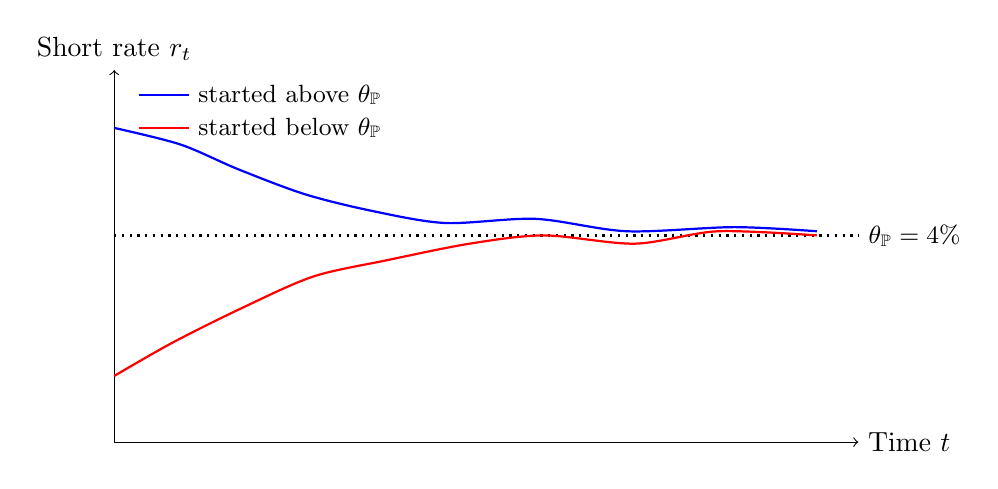
\begin{tikzpicture}[scale=1.05]
  \draw[->](0,0)--(9,0) node[right]{Time $t$};
  \draw[->](0,0)--(0,4.5) node[above]{Short rate $r_t$};
  \draw[dotted,thick](0,2.5)--(9,2.5) node[right]{\small$\theta_\PP=4\%$};
  % path starting above
  \draw[thick,blue] plot[smooth] coordinates
    {(0,3.8)(0.8,3.6)(1.5,3.3)(2.3,3.0)(3.1,2.8)(4.0,2.65)(5.1,2.7)(6.2,2.55)(7.5,2.6)(8.5,2.55)};
  % path starting below
  \draw[thick,red] plot[smooth] coordinates
    {(0,0.8)(0.7,1.2)(1.5,1.6)(2.4,2.0)(3.3,2.2)(4.3,2.4)(5.2,2.5)(6.3,2.4)(7.3,2.55)(8.5,2.5)};
  % legend
  \draw[blue,thick](0.3,4.2)--(0.9,4.2); \node[right] at (0.9,4.2){\small started above $\theta_\PP$};
  \draw[red,thick](0.3,3.8)--(0.9,3.8); \node[right] at (0.9,3.8){\small started below $\theta_\PP$};
\end{tikzpicture}
\caption{Qualitative CIR sample paths.  Both paths revert toward $\theta_\PP$
(dashed line), but with stochastic fluctuations.  Paths starting above
$\theta_\PP$ drift downward; those starting below drift upward.  Volatility
is lower near the origin because of the $\sqrt{r_t}$ factor.}
\end{figure}

\subsection*{Open-ended questions}
\begin{itemize}
  \item The CIR model has only one factor ($r_t$).  Real yield curves move
  in three dimensions (level, slope, curvature).  How would a
  two-factor extension look, and what would the second factor represent?
  \item In recent years (2014-2021 in Europe), short rates were genuinely
  negative.  What does that imply about the CIR model as an empirical
  description of those markets?
\end{itemize}

\newpage
%============================================================
\section{Question 4: Risk-neutral dynamics under $\QQ$}
%============================================================

\subsection{Why do we need a different measure?}

We have described $r_t$ under $\PP$ -- the measure that reflects actual
probabilities.  But pricing a bond requires computing an expectation of a
future payoff.  The question is: under \emph{which} probability measure?

The answer from no-arbitrage theory -- which we established in class
through the first fundamental theorem of asset pricing -- is that prices
of traded assets must be \emph{martingales under some equivalent probability
measure} $\QQ$ (after discounting by the money-market account).

\begin{recall_box}
From Definition 14 (Reminder sheet), a process $M_t$ is a
$\QQ$-\textbf{martingale} if $\EE_s^\QQ[M_t] = M_s$ for $s<t$.

From Definition 23, a \textbf{martingale measure} (risk-neutral measure)
$\QQ$ is an equivalent probability measure under which every discounted
traded asset is a martingale.

``Equivalent'' means $\QQ$ and $\PP$ agree on which events are possible
(zero-probability sets coincide), but they assign different probabilities
to non-null events.
\end{recall_box}

\subsection{The Radon-Nikodym derivative: the ``exchange rate'' between measures}

Since $\QQ$ and $\PP$ are equivalent, there exists a positive random
variable $\frac{\dd\QQ}{\dd\PP}$ (the \textbf{Radon-Nikodym derivative})
such that for any random variable $X$:
\[
\EE^\QQ[X] = \EE^\PP\!\left[X \cdot \frac{\dd\QQ}{\dd\PP}\right].
\]
Think of $\frac{\dd\QQ}{\dd\PP}(\omega)$ as the ``weight'' that adjusts
$\PP$-probabilities to $\QQ$-probabilities at each scenario $\omega$.
Scenarios where $\QQ$ assigns more probability than $\PP$ have weight
$>1$; scenarios where $\QQ$ assigns less have weight $<1$.

\subsection{Girsanov's theorem: the bridge between $\PP$ and $\QQ$}

\textbf{Girsanov's theorem} (in continuous time) says: given a process
$(\lambda_t)_{t\ge 0}$ satisfying certain integrability conditions, we can
define a new measure $\QQ$ via:
\[
\frac{\dd\QQ}{\dd\PP}\bigg|_{\FF_T}
= Z_T,
\quad
Z_t = \exp\!\left(-\int_0^t \lambda_s\,\dd W_s^\PP - \tfrac{1}{2}\int_0^t \lambda_s^2\,\dd s\right).
\]
Under $\QQ$, the process
\[
W_t^\QQ := W_t^\PP + \int_0^t \lambda_s\,\dd s
\]
is a standard Brownian motion.

\textbf{In English:} we take the $\PP$-Brownian motion and add a drift to
it.  The new process $W_t^\QQ$ is a genuine Brownian motion under $\QQ$,
but from the $\PP$ perspective it has a drift $-\lambda_t\,\dd t$ subtracted.
The parameter $\lambda_t$ is called the \textbf{market price of risk}: it
tells you how much drift the market demands for bearing one unit of
Brownian risk.

\subsection{From $\PP$ to $\QQ$: rewriting the CIR SDE}

Under $\PP$:
\[
\dd r_t = \kappa_\PP(\theta_\PP - r_t)\,\dd t + \sigma\sqrt{r_t}\,\dd W_t^\PP.
\]
Since $\dd W_t^\PP = \dd W_t^\QQ - \lambda_t\,\dd t$ (from Girsanov):
\[
\dd r_t
= \kappa_\PP(\theta_\PP - r_t)\,\dd t
+ \sigma\sqrt{r_t}(\dd W_t^\QQ - \lambda_t\,\dd t)
= \big[\kappa_\PP(\theta_\PP - r_t) - \sigma\sqrt{r_t}\lambda_t\big]\dd t
+ \sigma\sqrt{r_t}\,\dd W_t^\QQ.
\]

We want this to look like a CIR model under $\QQ$:
\[
\dd r_t = \kappa_\QQ(\theta_\QQ - r_t)\,\dd t + \sigma\sqrt{r_t}\,\dd W_t^\QQ.
\]
(Note: the $\sigma$ is the same under both measures -- Girsanov only changes
the drift, not the diffusion coefficient.)

\subsection{(ii) The required functional form of $\lambda_t$}

For the $\QQ$-drift to be of the form $\kappa_\QQ(\theta_\QQ - r_t)$ (affine in $r_t$), we need
\[
\kappa_\PP(\theta_\PP - r_t) - \sigma\sqrt{r_t}\lambda_t
= \kappa_\QQ\theta_\QQ - \kappa_\QQ r_t.
\]
Rearranging:
\[
\sigma\sqrt{r_t}\lambda_t
= (\kappa_\PP - \kappa_\QQ)r_t + (\kappa_\PP\theta_\PP - \kappa_\QQ\theta_\QQ).
\]
The right-hand side must be expressible as $\sigma\sqrt{r_t}\lambda_t$.
For this to hold for all $r_t > 0$, we need $\lambda_t$ of the form:
\[
\lambda_t = \frac{(\kappa_\PP-\kappa_\QQ)r_t + (\kappa_\PP\theta_\PP - \kappa_\QQ\theta_\QQ)}{\sigma\sqrt{r_t}}
= \underbrace{\frac{\kappa_\PP\theta_\PP - \kappa_\QQ\theta_\QQ}{\sigma\sqrt{r_t}}}_{\text{term 1}}
+ \underbrace{\frac{\kappa_\PP - \kappa_\QQ}{\sigma}\sqrt{r_t}}_{\text{term 2}}.
\]

The most common special case (and the standard CIR market price of risk)
sets the term 1 to zero (to avoid singularity at $r_t=0$):
\[
\kappa_\PP\theta_\PP = \kappa_\QQ\theta_\QQ,
\quad
\lambda_t = \frac{\kappa_\PP - \kappa_\QQ}{\sigma}\sqrt{r_t} =: \eta\sqrt{r_t}.
\]
In this case:
\[
\kappa_\QQ = \kappa_\PP + \sigma\eta,
\qquad
\kappa_\QQ\theta_\QQ = \kappa_\PP\theta_\PP.
\]

\begin{intuition}
The market price of risk $\lambda_t = \eta\sqrt{r_t}$ says: \emph{the
compensation for bearing interest rate risk is proportional to the square
root of the current rate}.  When rates are high (stressful times for
bondholders), the market demands a higher risk premium.  When rates are
near zero, the risk premium is also near zero (there is little systematic
risk in a near-zero rate environment).  This state-dependence is what
makes the CIR risk premium economically sensible.
\end{intuition}

\subsection{(i) The link between $(\kappa_\PP,\theta_\PP)$ and $(\kappa_\QQ,\theta_\QQ)$}

Collecting the results:
\[
\boxed{
\kappa_\QQ = \kappa_\PP + \sigma\eta,
\qquad
\theta_\QQ = \frac{\kappa_\PP\theta_\PP}{\kappa_\PP + \sigma\eta}.
}
\]

Several important observations:

\begin{enumerate}
  \item If $\eta > 0$ (risk aversion: investors accept lower returns
  for safety), then $\kappa_\QQ > \kappa_\PP$: mean reversion is
  \emph{faster} under $\QQ$ than under $\PP$.  Under $\QQ$, rates appear
  to pull toward the long-run level more quickly because the risk-neutral
  pricing already ``looks through'' the risk premium.

  \item The long-run levels satisfy:
  $\kappa_\QQ\theta_\QQ = \kappa_\PP\theta_\PP$ (constant product).  So if
  $\kappa_\QQ > \kappa_\PP$ then $\theta_\QQ < \theta_\PP$: the
  risk-neutral long-run level is \emph{lower} than the physical one.
  This is the risk premium compressed into the long end of the yield
  curve.

  \item $\eta$ is called the \textbf{price of risk} coefficient.  It is
  \emph{not} directly observable from market data.  To identify it, you
  need \emph{both} historical time series data (to get $\kappa_\PP,\theta_\PP$)
  \emph{and} bond or derivative prices (to get $\kappa_\QQ,\theta_\QQ$).
\end{enumerate}

\begin{example_box}
If $\kappa_\PP=0.3$, $\theta_\PP=0.04$, $\sigma=0.05$, and $\eta=1.0$:
\[
\kappa_\QQ = 0.3 + 0.05\times 1.0 = 0.35,
\quad
\theta_\QQ = \frac{0.3\times 0.04}{0.35} \approx 0.0343 = 3.43\%.
\]
So the risk-neutral long-run level is 3.43\%, which is below the physical
4\%.  The difference (57 basis points) represents the term premium embedded
in long-maturity yields.  This is why the risk-neutral yield curve tends
to be ``flatter'' than the physical expectations component: the risk premium
adds slope under $\PP$ that disappears under $\QQ$.
\end{example_box}

\subsection{(iii) Proving the Novikov condition}

\paragraph{What is the Novikov condition and why does it matter?}
We defined the Radon-Nikodym derivative $Z_T$ earlier.  For $Z_T$ to
define a \emph{valid} probability measure $\QQ$, we need $Z_T$ to be a
true martingale (not just a local martingale).  If $Z_T$ is only a local
martingale, then $\EE^\PP[Z_T]$ could be strictly less than 1, meaning
``probability mass is lost'' and $\QQ$ is not a proper probability measure.

The \textbf{Novikov condition} (Novikov, 1972) provides a simple sufficient
condition:
\[
\EE^\PP\!\left[\exp\!\left(\frac{1}{2}\int_0^T \lambda_t^2\,\dd t\right)\right]
< \infty.
\]
If this holds, then $Z_t$ is a true martingale and $\QQ$ is a valid
probability measure.

\paragraph{Why is Novikov checking the ``right'' thing?}
The process $Z_t$ involves a stochastic integral $\int_0^t \lambda_s\,\dd W_s^\PP$
plus a compensating drift $-\frac{1}{2}\int_0^t\lambda_s^2\,\dd s$.
The stochastic integral part is automatically a local martingale.  The
issue is whether it is a true (global) martingale.  Novikov's condition
checks that the ``size'' of the integrand $\lambda_t$ (measured by
$\int_0^T\lambda_t^2\,\dd t$) is not so large that probability mass leaks
to infinity.

\paragraph{Verifying Novikov for $\lambda_t = \eta\sqrt{r_t}$.}
With this choice:
\[
\frac{1}{2}\int_0^T \lambda_t^2\,\dd t
= \frac{\eta^2}{2}\int_0^T r_t\,\dd t.
\]
We need to show:
\[
\EE^\PP\!\left[\exp\!\left(\frac{\eta^2}{2}\int_0^T r_t\,\dd t\right)\right]
< \infty.
\]
The CIR process is an \textbf{affine process}, which means that its moment
generating function for functionals of the form $\int_0^T r_t\,\dd t$ is
exponential-affine in $r_0$:
\[
\EE^\PP\!\left[\exp\!\left(u\int_0^T r_t\,\dd t\right)\right]
= \exp\!\big(\alpha(T;u) + \beta(T;u)\,r_0\big),
\]
provided the Riccati ODEs for $(\alpha,\beta)$ have a solution on $[0,T]$.
This solution exists for $u < u^\star$ where $u^\star$ depends on $\kappa_\PP$
and $\sigma$.  Since $u = \eta^2/2$ is fixed, for any finite $T$ and
reasonable $\eta$ the Novikov integral is finite.  Therefore the Novikov
condition is satisfied on finite horizons.

\begin{intuition}
In plain terms: since $r_t$ is a non-negative, mean-reverting process that
cannot grow without bound, the integral $\int_0^T r_t\,\dd t$ is a.s.\
finite and cannot explode.  The exponential of this integral is finite in
expectation because the tails of the CIR distribution are sub-Gaussian for
reasonable parameters.  Contrast this with a process that can run away to
infinity, for which Novikov could fail.
\end{intuition}

\subsection{(iv) Why maintain the same structural specification under $\QQ$?}

\paragraph{First: what does ``not directly observable under $\QQ$'' mean?}
The measure $\QQ$ is a mathematical construction: it is not what you
observe when you watch the economy.  Time series of bond prices and rate
data are generated by the real world -- by $\PP$.  The risk-neutral measure
$\QQ$ exists as a pricing tool, but there is no direct way to estimate
$\QQ$-probabilities from historical data.

To see this, consider the following.  Under $\QQ$, the expected return on
every asset equals the risk-free rate $r_t$ (that is the definition of
$\QQ$).  But in reality, riskier assets earn higher expected returns under
$\PP$ (the equity premium, the term premium, etc.).  So if you tried to
use historical average returns to infer $\QQ$-expected returns, you would
get the wrong answer.

\paragraph{So why keep the same CIR structure?}
The compelling reason is \textbf{parsimony and tractability}:
\begin{enumerate}
  \item \textbf{One state variable, two measures.}  There is one object
  that drives interest rates: the short rate $r_t$.  It exists in the real
  world and is observed (approximately, through LIBOR, Fed Funds, OIS, etc.).
  Under $\PP$ and $\QQ$ it follows the same type of diffusion (CIR), just
  with different drift parameters.  This is elegant and consistent.

  \item \textbf{Closed-form bond prices.}  The CIR structure under $\QQ$
  (affine drift, square-root diffusion) is exactly what allows us to
  derive the log-affine bond pricing formula in Question 6.  If we changed
  the structure under $\QQ$ (e.g., made the diffusion coefficient $\sigma r_t$
  instead of $\sigma\sqrt{r_t}$), we would lose tractability.

  \item \textbf{Stable calibration.}  Keeping the CIR form under $\QQ$
  means we have only three parameters $(\kappa_\QQ, \theta_\QQ, \sigma)$
  to calibrate to cross-sectional bond prices.  This is manageable.

  \item \textbf{Theoretical coherence.}  The Girsanov change only changes
  the drift, not the diffusion.  So if you start with a CIR diffusion
  $(\sigma\sqrt{r_t})$ under $\PP$, it is \emph{automatic} that the
  diffusion remains $\sigma\sqrt{r_t}$ under $\QQ$ -- only the drift
  $\kappa_\PP(\theta_\PP-r_t)$ changes.  Maintaining the same structural
  form is not an assumption -- it is a consequence of the specific
  market price of risk $\lambda_t = \eta\sqrt{r_t}$.
\end{enumerate}

\paragraph{Effect of the measure change on expectations and variance.}
The change from $\PP$ to $\QQ$ affects the drift of $r_t$ but not its
diffusion:
\begin{align*}
\EE^\QQ[r_t \mid r_0] &= \theta_\QQ + (r_0-\theta_\QQ)e^{-\kappa_\QQ t}
\quad \text{(different from $\PP$ expectation)},\\
\mathrm{Var}^\QQ(r_t) &=
\frac{\sigma^2 r_0}{\kappa_\QQ}e^{-\kappa_\QQ t}(1-e^{-\kappa_\QQ t})
+\frac{\sigma^2\theta_\QQ}{2\kappa_\QQ}(1-e^{-\kappa_\QQ t})^2
\quad \text{(different scale, same structure)}.
\end{align*}
The \emph{local} variance (the diffusion coefficient squared times $\dd t$)
$\sigma^2 r_t\,\dd t$ is the same under both measures.  Only the
\emph{conditional mean} changes.

\subsection*{Open-ended questions}
\begin{itemize}
  \item If $\eta < 0$ (risk-seeking behaviour, or unusual environments like
  post-2008), what happens to $\kappa_\QQ$ and $\theta_\QQ$?  Does the
  Feller condition under $\QQ$ survive?
  \item How would you estimate $\eta$ empirically?  What data would you use?
\end{itemize}

\newpage
%============================================================
\section{Question 5: The discounted bond price is a $\QQ$-martingale}
%============================================================

\subsection{Setup and what we want to prove}

\begin{recall_box}
From Definition 14 (Reminder sheet), a process $M$ is a
$\QQ$-\textbf{martingale} on $(\Omega,\FF,(\FF_t),\QQ)$ if:
\begin{enumerate}
  \item $\EE^\QQ[|M_t|] < \infty$ for all $t$,
  \item $M_t$ is $\FF_t$-measurable (adapted) for all $t$,
  \item For all $s \le t$: $\EE^\QQ[M_t \mid \FF_s] = M_s$.
\end{enumerate}
The third property is the key one: the best forecast of a martingale's
future value, given current information, is its current value.  There is
no predictable drift.
\end{recall_box}

We want to show that the \textbf{discounted bond price}
\[
\widetilde{P}(t,T) := \frac{P(t,T)}{B_t}
= P(t,T)\exp\!\left(-\int_0^t r_s\,\dd s\right)
\]
is a $\QQ$-martingale.

\subsection{Why this should be true: the no-arbitrage argument}

Before the formal proof, let us understand why this must hold.

$B_t$ is the money-market account: if you invest \$1 at time 0 and earn the
risk-free short rate continuously, you accumulate $B_t$ by time $t$.  It is
the ``benchmark'' or ``numeraire''.

If $\widetilde{P}(t,T) = P(t,T)/B_t$ were \emph{not} a martingale under
$\QQ$, there would exist times $s < t$ for which $\EE^\QQ[\widetilde{P}(t,T)
\mid \FF_s] \ne \widetilde{P}(s,T)$.  But this would mean:
\begin{itemize}
  \item If $\EE^\QQ[\widetilde{P}(t,T)\mid\FF_s] > \widetilde{P}(s,T)$:
  the discounted bond ``earns more than the risk-free rate'' on average
  under $\QQ$ -- an arbitrage.
  \item If $\EE^\QQ[\widetilde{P}(t,T)\mid\FF_s] < \widetilde{P}(s,T)$:
  the discounted bond ``earns less than the risk-free rate'' -- you would
  short it and earn a riskless profit.
\end{itemize}
So the martingale property is equivalent to the no-arbitrage condition
for the bond market.

\subsection{The proof}

\textbf{Step 1: Write the bond price as a risk-neutral expectation.}

By the risk-neutral pricing formula (the definition of $\QQ$ in this
context):
\[
P(t,T) = \EE_t^\QQ\!\left[\exp\!\left(-\int_t^T r_u\,\dd u\right)\right]
= \EE^\QQ\!\left[\exp\!\left(-\int_t^T r_u\,\dd u\right)\bigg|\FF_t\right].
\]
This says: the bond price at $t$ is the $\QQ$-expected value of the
discount factor $e^{-\int_t^T r_u\,\dd u}$ (the ``stochastic discount
factor'' from $t$ to $T$), given all information up to $t$.

\textbf{Step 2: Write the discounted bond price.}

Multiply both sides by $B_t^{-1} = e^{-\int_0^t r_u\,\dd u}$:
\[
\widetilde{P}(t,T)
= e^{-\int_0^t r_u\,\dd u}\cdot\EE^\QQ\!\left[e^{-\int_t^T r_u\,\dd u}\bigg|\FF_t\right].
\]
Since $e^{-\int_0^t r_u\,\dd u}$ is $\FF_t$-measurable (it depends only
on information up to $t$), we can pull it inside the conditional expectation
(using property EC6 from the class notes: if $Y$ is $\FF_t$-measurable,
then $\EE^\QQ[XY|\FF_t] = Y\EE^\QQ[X|\FF_t]$):
\[
\widetilde{P}(t,T)
= \EE^\QQ\!\left[e^{-\int_0^t r_u\,\dd u}\cdot e^{-\int_t^T r_u\,\dd u}\bigg|\FF_t\right]
= \EE^\QQ\!\left[e^{-\int_0^T r_u\,\dd u}\bigg|\FF_t\right]
= \EE^\QQ\!\left[B_T^{-1}\bigg|\FF_t\right].
\]

\textbf{Step 3: Apply the tower property.}

Now take $s \le t$ and compute $\EE^\QQ[\widetilde{P}(t,T)\mid\FF_s]$:
\[
\EE^\QQ\!\left[\widetilde{P}(t,T)\bigg|\FF_s\right]
= \EE^\QQ\!\left[\EE^\QQ\!\left[B_T^{-1}\bigg|\FF_t\right]\bigg|\FF_s\right].
\]
Applying the \textbf{tower property of conditional expectation} (property EC3
from the Reminder: $\EE^\PP[\EE^\PP[X|\FF_t]|\FF_s] = \EE^\PP[X|\FF_s]$
when $s\le t$, and the same holds under $\QQ$):
\[
\EE^\QQ\!\left[\EE^\QQ\!\left[B_T^{-1}\bigg|\FF_t\right]\bigg|\FF_s\right]
= \EE^\QQ\!\left[B_T^{-1}\bigg|\FF_s\right]
= \widetilde{P}(s,T).
\]

\textbf{Conclusion:} For all $0 \le s \le t \le T$,
\[
\EE^\QQ\!\left[\widetilde{P}(t,T)\bigg|\FF_s\right] = \widetilde{P}(s,T).
\]
This is exactly the martingale property (condition M3 from Definition 14).
The discounted bond price is a $\QQ$-martingale. $\square$

\subsection{Financial interpretation of each step}

\begin{itemize}
  \item \textbf{Step 1} expresses the fundamental risk-neutral pricing
  principle: prices are $\QQ$-expectations of discounted payoffs.  Under $\QQ$,
  there is no risk premium -- all assets grow at the risk-free rate in
  expectation.
  \item \textbf{Step 2} combines the discount factor from $[0,t]$ (which we
  already know) with the stochastic discount factor from $[t,T]$ (which is
  still random at time $s$).  The product $e^{-\int_0^T r_u\,\dd u}$ is the
  total discount from $0$ to $T$.
  \item \textbf{Step 3} is the key probability-theoretic step: the tower
  property says ``if you first compute the best estimate given $\FF_t$ and
  then refine it given $\FF_s \subseteq \FF_t$, you get the same as directly
  computing the best estimate given $\FF_s$''.  This is the iterated
  expectations principle from your class notes.
\end{itemize}

\subsection{The SDE form of the martingale}

Since $\widetilde{P}$ is a $\QQ$-martingale and is continuous, it can be
written as a stochastic integral (by the Martingale Representation
Theorem):
\[
\dd\widetilde{P}(t,T) = \widetilde{P}(t,T)\cdot\Sigma(t,T)\,\dd W_t^\QQ
\]
for some adapted process $\Sigma(t,T)$ (the ``bond volatility'').  The
drift is zero, confirming the martingale property.  We will compute
$\Sigma(t,T)$ explicitly in Question 6.

\subsection*{Open-ended questions}
\begin{itemize}
  \item Can you give a direct proof (without going through the risk-neutral
  pricing formula) using the SDE for $P(t,T)$ derived in Question 6?
  \item What changes in the proof if $r_t$ can be negative?
\end{itemize}

\newpage
%============================================================
\section{Question 6: Zero-coupon bond price in log-affine form (CIR)}
%============================================================

\subsection{The pricing formula and what we are computing}

We want to find the explicit formula for:
\[
P(t,T)
= \EE_t^\QQ\!\left[\exp\!\left(-\int_t^T r_s\,\dd s\right)\right].
\]

Let us carefully unpack this before computing it.

\begin{itemize}
  \item $\exp\!\left(-\int_t^T r_s\,\dd s\right)$ is the \textbf{stochastic
  discount factor}: it discounts \$1 paid at $T$ back to time $t$ using the
  random short rate path.  If rates are high over $[t,T]$, this factor is
  small (heavy discounting).  If rates are low, it is closer to 1.

  \item $\EE_t^\QQ[\cdot]$ means we are taking the expectation under the
  risk-neutral measure $\QQ$, conditional on $\FF_t$ (everything known at
  time $t$, in particular $r_t$).

  \item Since $r_t$ is a Markov process, $P(t,T)$ depends on the history
  $(r_s)_{s\le t}$ \emph{only through the current value $r_t$}.  So we can
  write $P(t,T) = p(t,r_t;T)$ for some deterministic function $p$.

  \item The \textbf{log-affine form} asserts:
  $\log p(t,r;T) = a(t,T) - b(t,T)\cdot r$, or equivalently,
  $P(t,T) = e^{a(t,T)-b(t,T)r_t}$.  This means the log-price is a
  simple linear function of the current rate.  When $r_t$ rises by 1 unit,
  $\log P$ falls by $b(t,T)$ units -- $b(t,T)$ is essentially the
  \textbf{duration} of the bond.
\end{itemize}

\subsection{The Feynman-Kac approach: from expectation to PDE}

Rather than computing the expectation directly (which would require knowing
the full distribution of $\int_t^T r_s\,\dd s$), we use the
\textbf{Feynman-Kac theorem} to convert the pricing problem into a
\emph{partial differential equation} (PDE).

\textbf{Feynman-Kac theorem} (informal statement): If $X_t$ is a diffusion
process and $f(t,x)$ solves a certain PDE, then
$f(t,X_t) = \EE\!\left[g(X_T)\exp\!\left(-\int_t^T c(s,X_s)\,\dd s\right)\bigg|\,X_t=x\right]$.

For our problem, $X_t = r_t$ (the CIR process under $\QQ$), $g\equiv 1$
(the payoff is \$1 at $T$), and $c(s,r) = r$ (the discount rate equals the
short rate).  The function $p(t,r) := P(t,T)$ then satisfies:

\[
\frac{\partial p}{\partial t}
+ \kappa_\QQ(\theta_\QQ - r)\frac{\partial p}{\partial r}
+ \frac{1}{2}\sigma^2 r\frac{\partial^2 p}{\partial r^2}
- r\cdot p = 0,
\]
with terminal condition $p(T,r) = 1$ for all $r \ge 0$.

Let us read this PDE term by term:
\begin{itemize}
  \item $\partial_t p$: how fast the price changes due to time passing
  (time decay).
  \item $\kappa_\QQ(\theta_\QQ-r)\partial_r p$: the drift of $r_t$ under
  $\QQ$ pushes the price.
  \item $\frac{1}{2}\sigma^2 r\,\partial_{rr} p$: the convexity correction
  from the stochastic diffusion (the It\^o correction term).
  \item $-r\cdot p$: the discounting at rate $r$ (the ``kill'' term).
\end{itemize}
The PDE says: the infinitesimal change in value (time decay + drift effect
+ convexity) exactly equals the interest accrued.  This is the continuous-time
analogue of the bond pricing identity $\partial V/\partial t = rV$ in
deterministic finance.

\subsection{(i) Proving the log-affine representation}

\paragraph{The ansatz.}  We guess that the solution takes the log-affine form:
\[
p(t,r;T) = \exp\!\big(a(\tau) - b(\tau)r\big),
\qquad \tau := T - t \ge 0.
\]
(We write $a(\tau)$ and $b(\tau)$ rather than $a(t,T)$ and $b(t,T)$ to
emphasise that they depend only on the time-to-maturity $\tau = T-t$, not
on $t$ and $T$ separately.)

\textbf{Why is this guess reasonable?}  In the deterministic case ($\sigma=0$),
the bond price would be $e^{-r\tau}$ (discounting at constant rate $r$).
Our guess generalises this by allowing the ``effective rate'' to be $b(\tau)r$
and adding an intercept $a(\tau)$.

\textbf{Boundary conditions at $\tau = 0$:}  $p(T,r;T)=1 = e^0$, so
$a(0) = 0$ and $b(0) = 0$.

\paragraph{Substituting into the PDE.}  Let $P = e^{a-br}$.  Compute each
derivative:
\begin{align*}
\frac{\partial P}{\partial t}
&= \frac{\partial P}{\partial\tau}\cdot\frac{\partial\tau}{\partial t}
= -(a'(\tau) - b'(\tau)r)\,P, \\
\frac{\partial P}{\partial r}
&= -b(\tau)\,P, \\
\frac{\partial^2 P}{\partial r^2}
&= b(\tau)^2\,P.
\end{align*}

Substituting into the PDE and dividing by $P > 0$:
\begin{align*}
-(a'-b'r)
+ \kappa_\QQ(\theta_\QQ - r)(-b)
+ \tfrac{1}{2}\sigma^2 r\cdot b^2 - r &= 0.
\end{align*}
Expanding:
\[
-a' + b'r - \kappa_\QQ\theta_\QQ b + \kappa_\QQ r b
+ \tfrac{1}{2}\sigma^2 b^2 r - r = 0.
\]
Grouping by powers of $r$:
\begin{align*}
\text{constant in } r:&\quad
-a' - \kappa_\QQ\theta_\QQ b = 0, \\
\text{linear in } r:&\quad
b' + \kappa_\QQ b + \tfrac{1}{2}\sigma^2 b^2 - 1 = 0.
\end{align*}

\paragraph{The ODE system.}  We have obtained two ODEs:

\begin{align}
b'(\tau) &= 1 - \kappa_\QQ b(\tau) - \tfrac{1}{2}\sigma^2 b(\tau)^2,
\qquad b(0) = 0, \label{eq:Riccati}\\
a'(\tau) &= \kappa_\QQ\theta_\QQ\,b(\tau),
\qquad a(0) = 0. \label{eq:Aode}
\end{align}

Equation \eqref{eq:Riccati} is a \textbf{Riccati ODE} (a first-order
nonlinear ODE of the form $y' = p + qy + ry^2$).  Equation \eqref{eq:Aode}
is just an integral once $b$ is known.

\paragraph{Solving the Riccati ODE.}  Define
$\gamma := \sqrt{\kappa_\QQ^2 + 2\sigma^2}$.  Note $\gamma > \kappa_\QQ > 0$.

The Riccati ODE \eqref{eq:Riccati} can be solved by substitution.  The
exact solution is:
\[
b(\tau) = \frac{2(e^{\gamma\tau}-1)}
{(\gamma+\kappa_\QQ)(e^{\gamma\tau}-1)+2\gamma}.
\]

Let us verify the boundary condition: at $\tau=0$, numerator is $0$ and
denominator is $2\gamma > 0$, so $b(0) = 0$. \checkmark

For small $\tau$: using $e^{\gamma\tau} \approx 1+\gamma\tau$,
$b(\tau) \approx \frac{2\gamma\tau}{2\gamma} = \tau$.  So at short
maturities, $b\approx\tau$ and $P(t,T)\approx e^{-r_t\tau}$ -- exactly
the deterministic discounting formula.  The CIR formula reduces to
deterministic discounting at short maturities.

\paragraph{Solving the $a$ ODE.}
Substituting and integrating:
\[
a(\tau)
= \kappa_\QQ\theta_\QQ\int_0^\tau b(u)\,\dd u
= \frac{2\kappa_\QQ\theta_\QQ}{\sigma^2}
\log\!\left(
\frac{2\gamma e^{(\kappa_\QQ+\gamma)\tau/2}}
{(\gamma+\kappa_\QQ)(e^{\gamma\tau}-1)+2\gamma}
\right).
\]

\paragraph{The result.}
\[
\boxed{
\log P(t,T) = a(T-t) - b(T-t)\,r_t,
}
\]
with $b$ and $a$ as above.  The zero-coupon yield is therefore:
\[
y(t,T) = -\frac{\log P(t,T)}{T-t} = \frac{b(T-t)}{T-t}\,r_t - \frac{a(T-t)}{T-t}.
\]
This is a linear function of $r_t$ -- the entire yield curve moves up and
down proportionally to $r_t$.

\begin{intuition}
The function $b(T-t)$ plays the role of \textbf{duration} in the CIR
model.  For short maturities, $b(\tau)\approx \tau$ -- the price is
approximately the deterministic discount factor.  As $\tau\to\infty$,
$b(\tau) \to \frac{2}{\gamma+\kappa_\QQ}$, a finite constant.  This means
that very long bonds have bounded sensitivity to $r_t$, unlike in a
Vasicek model where $b(\tau)\to\infty$.  This is the mean reversion in
action: the CIR model ``caps'' the interest rate sensitivity of very long
bonds.
\end{intuition}

\begin{example_box}
With $\kappa_\QQ=0.35$, $\sigma=0.05$, $\theta_\QQ=0.0343$:
\[
\gamma = \sqrt{0.35^2 + 2\times0.0025} = \sqrt{0.1225+0.005} = \sqrt{0.1275} \approx 0.357.
\]
For $\tau = 5$ years and $r_0 = 0.02$:
\[
b(5) = \frac{2(e^{0.357\times5}-1)}{(0.357+0.35)(e^{1.785}-1)+2\times0.357}
= \frac{2(5.96-1)}{0.707\times 4.96 + 0.714}
\approx \frac{9.92}{4.22}\approx 2.35.
\]
So $\log P(0,5) = a(5) - 2.35\times 0.02 \approx a(5) - 0.047$.
The five-year yield is $y(0,5) = 2.35/5\times r_0 - a(5)/5$.
\end{example_box}

\subsection{(ii) SDE satisfied by $P(t,T)$}

Now we use It\^o's lemma on $P(t,T) = e^{a(\tau)-b(\tau)r_t}$ where
$\tau = T-t$ is decreasing in $t$.

Under $\QQ$, $r_t$ satisfies:
\[
\dd r_t = \kappa_\QQ(\theta_\QQ-r_t)\,\dd t + \sigma\sqrt{r_t}\,\dd W_t^\QQ.
\]
Applying It\^o's formula to $f(t,r_t) = e^{a(T-t)-b(T-t)r_t}$:
\[
\dd P = \left(\partial_t P + \kappa_\QQ(\theta_\QQ-r_t)\partial_r P
+ \tfrac{1}{2}\sigma^2 r_t\partial_{rr}P\right)\dd t
+ \partial_r P\cdot\sigma\sqrt{r_t}\,\dd W_t^\QQ.
\]
The PDE tells us that the $\dd t$ bracket equals $r_t P$.  And
$\partial_r P / P = -b(t,T)$.  Hence:
\[
\frac{\dd P(t,T)}{P(t,T)}
= r_t\,\dd t - \sigma b(t,T)\sqrt{r_t}\,\dd W_t^\QQ.
\]
Or equivalently:
\[
\dd P(t,T) = P(t,T)\big[r_t\,\dd t - \sigma b(t,T)\sqrt{r_t}\,\dd W_t^\QQ\big].
\]

\textbf{Reading this equation:}
\begin{itemize}
  \item The drift of the bond under $\QQ$ is $r_t\,\dd t$ -- the bond
  earns exactly the risk-free rate.  This is precisely the martingale
  condition: after discounting by $B_t$, no systematic gain remains.
  \item The volatility of the bond is $\sigma b(t,T)\sqrt{r_t}$.  This is:
  \begin{itemize}
    \item proportional to $b(t,T)$: longer-maturity bonds (larger $b$) are
    more volatile,
    \item proportional to $\sqrt{r_t}$: bond volatility is higher when rates
    are higher,
    \item proportional to $\sigma$: the parameter $\sigma$ controls how much
    bond prices fluctuate.
  \end{itemize}
\end{itemize}

\subsection*{Open-ended questions}
\begin{itemize}
  \item As $T\to\infty$, what does the yield $y(0,T)$ converge to in the CIR
  model?  Is this a reasonable long-run yield level?
  \item If we observed two bonds of different maturities, could we identify
  $\kappa_\QQ$, $\theta_\QQ$, and $\sigma$ from their prices alone?
  How many bonds do you need?
\end{itemize}

\newpage
%============================================================
\section{Question 7: Fitting the initial yield curve}
%============================================================

\subsection{The problem: three parameters are not enough}

We have a model $(\kappa_\QQ,\theta_\QQ,\sigma)$ with three parameters.
Once we fix $r_0$ (today's short rate), the model completely determines the
entire yield curve $T\mapsto y^{model}(0,T)$ via the CIR formula.  But the
real market gives us a yield $y^{market}(0,T)$ for every maturity $T$, and
in general:
\[
y^{model}(0,T) \ne y^{market}(0,T) \qquad \text{for most $T$}.
\]

This is a serious problem.  If the model misprices the initial yield curve,
it will also misprice derivatives (since their prices are functions of bond
prices).  A \textbf{term structure model that cannot even match today's market}
is not fit for use in derivatives pricing.

\begin{intuition}
Think of it this way.  The yield curve on any given day has a complex,
irregular shape -- perhaps humped at the 5-year point, with a kink at 30
years due to pension fund demand.  A three-parameter family of curves
(CIR) cannot match all these features exactly.  It is like trying to fit
an arbitrary polynomial with only a quadratic -- you can get the general
shape, but not every detail.
\end{intuition}

\subsection{The remedy: time-dependent $\theta_t^\QQ$}

The standard fix (Hull and White, 1990; applied to CIR by Rogers, 1995) is
to replace the constant long-run mean $\theta_\QQ$ with a
\textbf{deterministic function of time} $\theta_t^\QQ$.  The modified
model is:
\[
\dd r_t = \kappa_\QQ\big(\theta_t^\QQ - r_t\big)\,\dd t
+ \sigma\sqrt{r_t}\,\dd W_t^\QQ, \qquad r_0 > 0.
\]

Now $\theta_t^\QQ$ is an entire function, giving us infinitely many degrees
of freedom.  We can choose it to match the initial yield curve exactly.

\textbf{What is preserved?}
\begin{itemize}
  \item The diffusion term $\sigma\sqrt{r_t}$ is unchanged.
  \item The affine structure is preserved: bond prices are still
  exponential-affine in $r_t$, so we retain tractability.
  \item The Feller positivity condition still holds locally (at each $t$,
  the local drift is $\kappa_\QQ\theta_t^\QQ > 0$ away from zero).
\end{itemize}

\textbf{What changes?}  The model is no longer time-homogeneous.
The coefficients $a(t,T)$ and $b(t,T)$ in the log-affine formula now
depend on the whole path of $\theta_u^\QQ$ for $u \in [t,T]$, not just
on $\tau = T-t$.

\subsection{Bond price formula with time-dependent $\theta_t^\QQ$}

The bond pricing PDE becomes:
\[
\partial_t p + \kappa_\QQ(\theta_t^\QQ - r)\partial_r p
+ \tfrac{1}{2}\sigma^2 r\partial_{rr}p - rp = 0,
\quad p(T,r) = 1.
\]

The ansatz $p = e^{A(t,T)-B(t,T)r}$ still works.  The $B$ equation is the
same Riccati ODE (independent of $\theta_t^\QQ$):
\[
-\partial_t B = 1 - \kappa_\QQ B - \tfrac{1}{2}\sigma^2 B^2,
\quad B(T,T) = 0.
\]
This can be rewritten in $\tau = T-t$: $b'(\tau) = 1 - \kappa_\QQ b -
\tfrac{1}{2}\sigma^2 b^2$ with $b(0)=0$ -- the same as before.  So $b(\tau)$
is unchanged.

The $A$ equation becomes:
\[
-\partial_t A = \kappa_\QQ\theta_t^\QQ B(t,T),
\quad A(T,T) = 0,
\]
which integrates to:
\[
A(0,T) = \kappa_\QQ\int_0^T \theta_u^\QQ\,b(T-u)\,\dd u.
\]

\subsection{Calibrating $\theta_t^\QQ$ to the initial curve}

At $t=0$, we observe the market yield curve $T\mapsto y^{mkt}(0,T)$, which
gives the market discount curve:
\[
P^{mkt}(0,T) = e^{-T\,y^{mkt}(0,T)}.
\]
The model must match: $P^{model}(0,T) = P^{mkt}(0,T)$ for all $T$.

Since $P^{model}(0,T) = \exp(A(0,T) - b(T)r_0)$ where we write
$b(T) := B(0,T)$ (the Riccati solution evaluated at $\tau=T$), matching
gives:
\[
A(0,T) = \log P^{mkt}(0,T) + b(T)r_0.
\]
Substituting the formula for $A$:
\[
\kappa_\QQ\int_0^T \theta_u^\QQ\,b(T-u)\,\dd u
= \log P^{mkt}(0,T) + b(T)r_0.
\]

Define $\Psi(T) := \log P^{mkt}(0,T) + b(T)r_0$.  This is a known
function of $T$ (computable from market data and the Riccati solution).
Then $\theta^\QQ$ must satisfy:
\[
\boxed{
\Psi(T) = \kappa_\QQ\int_0^T \theta_u^\QQ\,b(T-u)\,\dd u.
}
\]
This is a \textbf{Volterra integral equation of the first kind}: it asks
``which function $\theta_u^\QQ$ produces a given convolution with $b$?''

\paragraph{Numerical recipe.}  On a maturity grid $0 = T_0 < T_1 < \cdots < T_n$:
\begin{enumerate}
  \item From market data, compute $P^{mkt}(0,T_i)$ and hence $\Psi(T_i)$.
  \item Solve the Riccati ODE for $b(T)$ on the grid (numerically if needed).
  \item Approximate the convolution integral using piecewise-constant
  $\theta_u^\QQ = \theta_{T_{k-1}}^\QQ$ for $u\in[T_{k-1},T_k)$.
  \item This turns the integral equation into a lower-triangular linear
  system, solvable sequentially: given $\theta$ values at earlier dates,
  solve for $\theta_{T_k}^\QQ$ at each new maturity.
\end{enumerate}

\begin{example_box}
\textbf{Illustrative two-point example.}  Suppose $r_0=0.02$, $\kappa_\QQ=0.35$, $\sigma=0.05$, and:
\[
P^{mkt}(0,1) = 0.980, \quad P^{mkt}(0,2) = 0.955.
\]
From the Riccati solution: $b(1)\approx 0.92$, $b(2)\approx 1.70$.

$\Psi(1) = \log(0.980) + 0.92\times0.02 \approx -0.0202 + 0.0184 = -0.0018$.

For the first interval, with piecewise-constant $\theta_u^\QQ = \theta_1$:
\[
\kappa_\QQ\theta_1\int_0^1 b(1-u)\,\dd u \approx 0.35\theta_1\times 0.45 \approx 0.158\theta_1 = -0.0018,
\]
so $\theta_1 \approx -0.011$.  (This negative value just illustrates the
sensitivity; with realistic market data the values are positive.)
\end{example_box}

\subsection{How do we get $\kappa$ and $\sigma$?}

The time-dependent $\theta_t^\QQ$ can absorb the initial curve for any
fixed $(\kappa_\QQ, \sigma)$.  So how do we choose $\kappa_\QQ$ and
$\sigma$?

\textbf{Route 1: Historical estimation.}  Use daily or weekly short-rate
data (e.g., 3-month T-bill yields as a proxy for $r_t$) to estimate the
$\PP$ parameters $(\kappa_\PP, \theta_\PP, \sigma)$.  Since $\sigma$ is
the same under $\PP$ and $\QQ$, this gives $\sigma$ directly.  For
$\kappa_\QQ$, you also need the market price of risk coefficient $\eta$,
which requires cross-sectional bond data.

\textbf{Route 2: Calibration to derivative prices.}  Fix $(\kappa_\QQ,\sigma)$
and minimise the pricing error across a panel of liquid cap/floor or
swaption prices.  Since these instruments are sensitive to $\sigma$ and
$\kappa_\QQ$ in distinct ways, the two parameters can in principle be
identified.

\begin{figure}[ht]
\centering
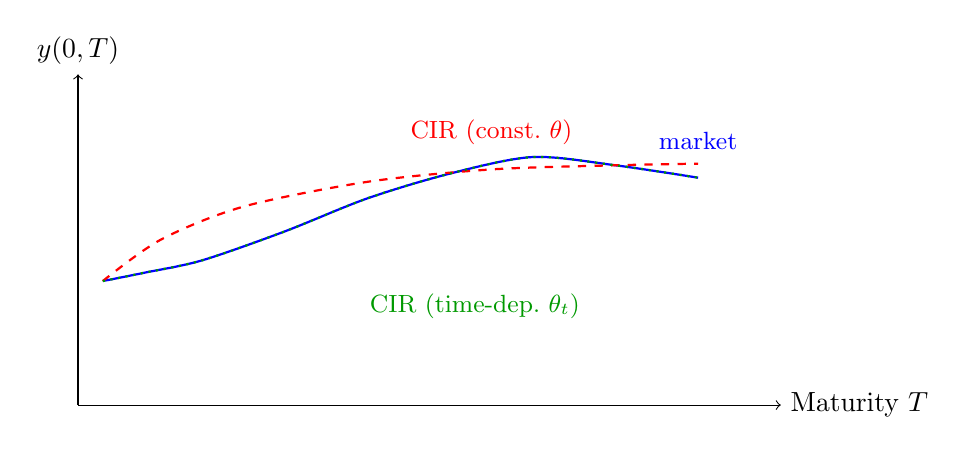
\begin{tikzpicture}[scale=1.05]
  \draw[->](0,0)--(8.5,0) node[right]{Maturity $T$};
  \draw[->](0,0)--(0,4.0) node[above]{$y(0,T)$};
  % market curve (irregular)
  \draw[thick,blue] plot[smooth] coordinates
    {(0.3,1.5)(0.8,1.6)(1.5,1.75)(2.5,2.1)(3.5,2.5)(4.5,2.8)(5.5,3.0)(6.5,2.9)(7.5,2.75)};
  % CIR constant theta curve
  \draw[thick,red,dashed] plot[smooth] coordinates
    {(0.3,1.5)(1.0,2.0)(2.0,2.4)(3.5,2.7)(5.0,2.85)(6.5,2.9)(7.5,2.92)};
  % CIR with time-dep theta (perfect fit)
  \draw[thick,green!60!black,dotted] plot[smooth] coordinates
    {(0.3,1.5)(0.8,1.6)(1.5,1.75)(2.5,2.1)(3.5,2.5)(4.5,2.8)(5.5,3.0)(6.5,2.9)(7.5,2.75)};
  \node[blue] at (7.5,3.2) {\small market};
  \node[red] at (5.0,3.3) {\small CIR (const.\ $\theta$)};
  \node[green!60!black] at (4.8,1.2) {\small CIR (time-dep.\ $\theta_t$)};
\end{tikzpicture}
\caption{Motivation for time-dependent $\theta_t^\QQ$.  The three-parameter CIR model
(dashed red) cannot replicate the hump in the market yield curve.  The
time-dependent extension (dotted green) fits exactly by construction.}
\end{figure}

\subsection*{Open-ended questions}
\begin{itemize}
  \item If $\theta_t^\QQ$ is calibrated daily to market data, what does the
  time series of $\theta_t^\QQ$ tell us about the market's risk-neutral
  expectations?
  \item Should we smooth $\theta_t^\QQ$ (e.g., constrain it to be a
  polynomial in $t$)?  What is the trade-off?
\end{itemize}

\newpage
%============================================================
\section{Question 8: Interest rate swaps}
%============================================================

\subsection{(i) What is an interest rate swap?}

\paragraph{The practical motivation.}

Imagine a company, call it ABC Corp, that has issued a \$100 million
floating-rate loan.  The interest payments reset every quarter and are
linked to the 3-month LIBOR rate.  ABC Corp is exposed to interest rate
risk: if LIBOR rises from 3\% to 6\%, their quarterly payments double.
The CFO wants to eliminate this uncertainty and pay a fixed amount each
quarter instead.

On the other side, a bank (XYZ Bank) has a fixed-rate mortgage portfolio
paying 5\% fixed.  The bank funds itself with short-term deposits paying a
floating rate.  If rates rise, the bank's funding cost rises but its
income is fixed -- a bad position.  The bank wants to \emph{receive} fixed
and \emph{pay} floating.

These two parties can enter an \textbf{interest rate swap (IRS)}: ABC pays
a fixed rate to XYZ and receives LIBOR, while XYZ pays LIBOR to ABC and
receives fixed.  After netting, ABC's effective obligation is fixed
(it pays fixed to XYZ and receives floating from XYZ which offsets its
loan), while XYZ has transformed its fixed income into floating income.

\paragraph{The formal definition.}

An \textbf{interest rate swap} is an OTC derivative contract between two
counterparties (call them the \emph{fixed-rate payer} and the
\emph{floating-rate payer}) to exchange cash flows on specified dates:
\begin{itemize}
  \item The \textbf{fixed leg}: a fixed interest rate $K$ applied to a
  notional $N$ over accrual periods $[T_{i-1}, T_i]$ for
  $i = a+1, \ldots, b$.
  \item The \textbf{floating leg}: a floating rate (in our model, set by
  the short rate) applied to $N$ over the same periods.
\end{itemize}

The payment dates are $T_{a+1},\ldots,T_b$, the swap starts at $T_a$
(the \emph{start date}), and we enter the swap at time $t \le T_a$.  We
write $\delta_i = T_i - T_{i-1}$ for the day-count fraction (accrual
period length).

\paragraph{Cash flows.}

For a \textbf{payer swap} (you pay fixed, receive floating):
\begin{itemize}
  \item At each date $T_i$: you \textbf{pay} $N K\delta_i$ (fixed).
  \item At each date $T_i$: you \textbf{receive} $N\big(e^{\int_{T_{i-1}}^{T_i}r_s\,\dd s}-1\big)$
  (floating, approximately $N r_{T_{i-1}}\delta_i$ in discrete terms).
\end{itemize}

\paragraph{The floating leg in terms of bond prices.}  In the
single-curve framework with continuous compounding, the floating leg
payment at $T_i$ (set at $T_{i-1}$) can be valued as:
\begin{align*}
N\big(P(t,T_{i-1}) - P(t,T_i)\big)
\end{align*}
because a floating payment at $T_i$ on notional $N$ over $[T_{i-1},T_i]$
equals a bond maturing at $T_{i-1}$ minus a bond maturing at $T_i$ (a
telescoping argument).

Summing over all periods, the total floating leg PV is:
\[
PV^{float}_t = N\big(P(t,T_a) - P(t,T_b)\big).
\]

\begin{intuition}
This telescoping is elegant and worth understanding.  The floating leg is
equivalent to: receive \$1 at $T_a$ and pay \$1 at $T_b$.  If you lend
\$1 at $T_a$ at the prevailing floating rate, you receive the floating
coupons and get \$1 back at $T_b$.  The PV of ``receive \$1 at $T_a$, pay
\$1 at $T_b$'' is exactly $P(t,T_a) - P(t,T_b)$.  The floating coupon
payments in between are the ``interest'' you earn, and they net out to this
difference.
\end{intuition}

The \textbf{fixed leg} PV is straightforward:
\[
PV^{fix}_t = NK\sum_{i=a+1}^{b}\delta_i P(t,T_i).
\]

\subsection{(ii) The swap rate}

\paragraph{Definition.}  The \textbf{par swap rate} (or simply \emph{swap rate}) at time $t$,
$S(t;T_a,T_b)$, is the fixed rate $K$ that makes the payer swap worth
zero at inception:
\[
V_t^{payer} = N\big(P(t,T_a)-P(t,T_b)\big) - NK\sum_{i=a+1}^b \delta_i P(t,T_i) = 0.
\]
Solving for $K$:
\[
\boxed{
S(t;T_a,T_b)
= \frac{P(t,T_a) - P(t,T_b)}{\sum_{i=a+1}^{b}\delta_i\,P(t,T_i)}.
}
\]

\paragraph{Economic interpretation.}

\begin{itemize}
  \item \textbf{Numerator} $P(t,T_a)-P(t,T_b)$: this is the PV of the
  floating leg.  It is the value of receiving \$1 at $T_a$ and paying \$1
  at $T_b$ -- the ``spread'' across the swap's life.

  \item \textbf{Denominator} $\sum_{i=a+1}^b\delta_i P(t,T_i)$: this is
  called the \textbf{swap annuity} or \textbf{DV01} (dollar value of 1
  basis point, scaled).  It is the PV of receiving 1 unit of currency per
  period over the swap's life.  It converts the ratio into an annualised
  rate.

  \item The swap rate is therefore: ``PV of floating leg divided by the
  annuity''.  In words: $S$ is the fixed rate that makes the fixed-leg PV
  equal the floating-leg PV.
\end{itemize}

\begin{example_box}
Suppose $t=0$, $T_a=0$, $T_b = 2$ years, annual payments ($\delta_1=\delta_2=1$),
and $P(0,1)=0.95$, $P(0,2)=0.88$.

\[
S(0;0,2) = \frac{P(0,0)-P(0,2)}{P(0,1)+P(0,2)}
= \frac{1-0.88}{0.95+0.88}
= \frac{0.12}{1.83} \approx 6.56\%.
\]

So the 2-year swap rate is 6.56\%.  This means: if you enter a 2-year
payer swap today paying 6.56\% fixed annually, the present value of the
fixed payments exactly equals the present value of the floating payments.
The swap costs nothing to enter (ignoring bid-ask spreads and counterparty
risk).
\end{example_box}

\paragraph{Swap rate as a function of ZCB prices.}  The formula above
makes this explicit: $S(t;T_a,T_b)$ is entirely determined by the
zero-coupon bond prices $P(t,T_a), P(t,T_{a+1}), \ldots, P(t,T_b)$ at
time $t$.  No additional information is needed.  In the CIR model, each
$P(t,T_i) = e^{a(T_i-t)-b(T_i-t)r_t}$, so the swap rate is a
deterministic function of $r_t$ alone.

\subsection*{Open-ended questions}
\begin{itemize}
  \item In reality, floating legs are linked to LIBOR/SOFR, not to the
  theoretical short rate.  How does this change the valuation?  (This is
  the ``multi-curve'' problem.)
  \item Is the swap rate $S(t;T_a,T_b)$ a martingale under some measure?
  If so, under which one?
\end{itemize}

\newpage
%============================================================
\section{Question 9: Swaptions}
%============================================================

\subsection{(i) What is a swaption?}

\paragraph{Financial motivation.}

Continuing our story from Question 8: ABC Corp wants to enter a swap in
2 years to hedge floating-rate exposure, but is not sure whether it will
actually need the hedge (perhaps its floating-rate debt may be refinanced
early).  ABC wants the \emph{right} -- but not the obligation -- to enter
the swap.  This is a \textbf{swaption}.

More concretely:
\begin{itemize}
  \item A \textbf{payer swaption} with expiry $T_a$ and strike $K$ gives
  the holder the right to \emph{enter} a payer swap (pay fixed $K$,
  receive floating) starting at $T_a$.
  \item The holder exercises if and only if the market swap rate
  $S(T_a;T_a,T_b) > K$: if rates have risen, the option to pay the lower
  fixed rate $K$ is valuable.
\end{itemize}

Swaptions are one of the most liquid interest rate derivative instruments.
They are used to hedge the optionality embedded in mortgages (prepayment
options) and callable bonds.

\paragraph{Formal definition.}

A \textbf{European payer swaption} with notional $N$, expiry $T_a$, swap
tenor $[T_a,T_b]$, payment dates $T_{a+1},\ldots,T_b$, and strike $K$
has payoff at $T_a$:
\[
\Pi_{T_a}^{pay}
= N\left(V_{T_a}^{payer}\right)^+
= N\!\left(P(T_a,T_a)-P(T_a,T_b)-K\sum_{i=a+1}^b\delta_i P(T_a,T_i)\right)^+.
\]
Since $P(T_a,T_a)=1$:
\[
\Pi_{T_a}^{pay}
= N\left(1-P(T_a,T_b)-K\sum_{i=a+1}^b\delta_i P(T_a,T_i)\right)^+.
\]
Using the annuity $A_{T_a} = \sum_{i=a+1}^b \delta_i P(T_a,T_i)$ and the
swap rate formula:
\[
\Pi_{T_a}^{pay}
= N\cdot A_{T_a}\cdot(S(T_a;T_a,T_b)-K)^+.
\]
This is an option on the swap rate $S$: a call option (for a payer swaption).

\subsection{(ii) Pricing formula}

\paragraph{General risk-neutral formula.}

The time-$t$ price of the payer swaption is:
\[
V_t^{pay}
= \EE_t^\QQ\!\left[
e^{-\int_t^{T_a}r_s\,\dd s}\,\Pi_{T_a}^{pay}
\right]
= N\cdot\EE_t^\QQ\!\left[
e^{-\int_t^{T_a}r_s\,\dd s}\cdot A_{T_a}\cdot(S(T_a;T_a,T_b)-K)^+
\right].
\]

\paragraph{The swap-annuity measure.}  Define the \textbf{annuity numeraire}:
\[
A_t := A(t;T_a,T_b) = \sum_{i=a+1}^b\delta_i P(t,T_i).
\]
Since $A_t$ is a traded (non-negative) asset, it can serve as a numeraire.
Under the corresponding \textbf{annuity measure} $\QQ^A$:
\[
V_t^{pay} = N\cdot A_t\cdot\EE_t^{\QQ^A}\!\big[(S(T_a;T_a,T_b)-K)^+\big].
\]
The swap rate $S(t;T_a,T_b) = (P(t,T_a)-P(t,T_b))/A_t$ is a
$\QQ^A$-\textbf{martingale} (because the numerator is the difference of
two prices and the denominator is the numeraire).  This is the theoretical
foundation for Black's formula.

\paragraph{Black's swaption formula.}

If we assume the swap rate is log-normally distributed under $\QQ^A$,
we obtain the \textbf{Black swaption formula}:
\[
V_t^{pay}
= N\cdot A_t\Big(S_t\,\Phi(d_1) - K\,\Phi(d_2)\Big),
\]
where $S_t := S(t;T_a,T_b)$ is today's swap rate and:
\[
d_{1,2}
= \frac{\ln(S_t/K) \pm \frac{1}{2}\sigma_{swap}^2(T_a-t)}
{\sigma_{swap}\sqrt{T_a-t}},
\]
and $\sigma_{swap}$ is the \textbf{swaption (Black) implied volatility}.

\begin{intuition}
Black's formula treats the swaption exactly like a call option on a stock
(the ``stock'' being the swap rate $S_t$), but with the bond annuity $A_t$
playing the role of the discount factor.  The formula is the fixed income
analogue of the Black-Scholes formula.  The market quotes swaptions in
terms of $\sigma_{swap}$ (implied vol), not in terms of dollar prices.
\end{intuition}

\paragraph{CIR pricing via Jamshidian's decomposition.}

In the CIR model (or any one-factor short-rate model), we can be more
precise.  The swaption payoff can be rewritten as a portfolio of bond
\emph{options}:

\begin{enumerate}
  \item Let coupon weights $c_i = K\delta_i$ for $i=a+1,\ldots,b-1$ and
  $c_b = 1 + K\delta_b$.  Then:
  \[
  \Pi_{T_a}^{pay}
  = N\left(1 - \sum_{i=a+1}^b c_i P(T_a,T_i)\right)^+.
  \]

  \item Since $P(T_a,T_i) = e^{a(T_i-T_a)-b(T_i-T_a)r_{T_a}}$ is a
  \emph{monotone decreasing} function of $r_{T_a}$ (in a one-factor model,
  all bond prices move together), there exists a unique \emph{critical rate}
  $r^\star$ such that:
  \[
  \sum_{i=a+1}^b c_i P(T_a,T_i;r^\star) = 1.
  \]

  \item \textbf{Jamshidian's trick}: the payoff is positive iff
  $r_{T_a} < r^\star$ (low rates make bond prices high and the swap
  in-the-money for the payer).  Define $K_i = P(T_a,T_i;r^\star)$ as the
  ``strike'' for the $i$-th bond option.  Then:
  \[
  \Pi_{T_a}^{pay}
  = N\sum_{i=a+1}^b c_i\Big(K_i - P(T_a,T_i)\Big)^+.
  \]
  This is a \emph{portfolio of put options on zero-coupon bonds}, with
  notional $Nc_i$ and strike $K_i$ for the $i$-th bond.

  \item Each zero-coupon bond option can be priced in closed form in the
  CIR model using the non-central chi-squared distribution (since
  $P(T_a,T_i)$ is a function of $r_{T_a}$, whose distribution is known
  exactly).
\end{enumerate}

The CIR payer swaption price is therefore:
\[
V_t^{pay}
= N\sum_{i=a+1}^{b} c_i\,\text{ZCBput}(t;\,T_a,T_i,K_i),
\]
where $\text{ZCBput}(t;\,T_a,T_i,K_i)$ is the time-$t$ price of a put
option on the $T_i$-maturity ZCB, with expiry $T_a$ and strike $K_i$,
priced using the CIR distribution.

\begin{example_box}
\textbf{What Jamshidian's trick achieves.}  Pricing an option on a coupon
bond directly requires knowing the joint distribution of
$P(T_a,T_{a+1}),\ldots,P(T_a,T_b)$.  In a multi-factor model, this is
complicated.  In a one-factor model like CIR, all these bond prices are
determined by the single state variable $r_{T_a}$, so the joint
distribution reduces to the univariate distribution of $r_{T_a}$ -- which
we know exactly (non-central chi-squared).  Jamshidian's decomposition is
only possible in a one-factor world.

This is one practical limitation of CIR: it cannot price swaptions and
caps consistently without implying a perfect correlation between all bond
maturities.  In reality, swaption skews and cap-floor basis suggest
multi-factor dynamics.
\end{example_box}

\subsection*{Open-ended questions}
\begin{itemize}
  \item Under what conditions does the Black swaption formula overstate or
  understate the CIR price?  When are they approximately equal?
  \item How would you calibrate the CIR model to a panel of swaptions
  $V^{pay}(T_a, T_b, K)$ for multiple $(T_a,T_b,K)$?  Is the system
  over- or under-determined?
\end{itemize}

\newpage
%============================================================
\section*{References and suggested reading}
%============================================================

\begin{itemize}
  \item Cox, J.C., Ingersoll, J.E., Ross, S.A.\ (1985): ``A Theory of
  the Term Structure of Interest Rates.''  \emph{Econometrica}, 53(2),
  385--407.  \textit{The original CIR paper.}
  \item Brigo, D.\ and Mercurio, F.\ (2006): \emph{Interest Rate Models ---
  Theory and Practice}.  Springer.  \textit{The definitive reference;
  see Chapters 3 (CIR), 6 (swaptions), and 12 (term structure fitting).}
  \item Filipovi\'{c}, D.\ (2009): \emph{Term-Structure Models}.
  Springer.  \textit{Rigorous mathematical treatment of affine models.}
  \item Shreve, S.\ (2004): \emph{Stochastic Calculus for Finance II}.
  Springer.  \textit{Chapter 9 covers interest rate models.}
  \item Jamshidian, F.\ (1989): ``An exact bond option formula.''
  \emph{Journal of Finance}, 44(1), 205--209.  \textit{Original paper for
  the decomposition in Question 9.}
  \item Hull, J.\ and White, A.\ (1990): ``Pricing interest rate derivative
  securities.''  \emph{Review of Financial Studies}, 3(4), 573--592.
  \textit{The source for time-dependent drift extension.}
  \item Yamada, T.\ and Watanabe, S.\ (1971): ``On the uniqueness of
  solutions of stochastic differential equations.''
  \emph{J.\ Math.\ Kyoto Univ.}, 11, 155--167.
  \textit{For the strong solution result in Question 3.}
\end{itemize}

\section*{Simulation and coding roadmap (iteration 2)}

When we move to the coding phase, the following tasks are planned:

\begin{enumerate}
  \item \textbf{CIR simulation under $\PP$:} Euler-Maruyama and Milstein
  schemes for the square-root diffusion.  Plot sample paths, histogram of
  $r_T$ vs.\ the theoretical non-central chi-squared density.
  \item \textbf{Yield curve generation:} Given CIR parameters, compute
  $b(\tau)$ and $a(\tau)$ on a maturity grid and plot the yield and
  forward curves.
  \item \textbf{Initial curve fitting:} Load a FRED yield curve for a
  chosen date.  Solve the Volterra equation numerically to find
  $\theta_t^\QQ$. Plot observed vs.\ fitted yield curve.
  \item \textbf{Swap rate surface:} Compute the swap rate $S(0;0,T)$ as a
  function of tenor $T$.
  \item \textbf{Swaption pricing:} Implement Jamshidian's decomposition
  and plot the swaption price as a function of strike and expiry.
  Compare with Black's formula.
\end{enumerate}

\end{document}
